\documentclass{beamer}
\usepackage{textcomp} %textrightarrow
\usetheme{Boadilla}
\title{Analisi stato dell'arte efficienza energetica sistemi embedded}
\author{Pietro Ghiglio}
\begin{document}
\titlepage

\begin{frame}
\frametitle{Osservazioni}
\begin{itemize}
\item Ottimizzare il tempo di esecuzione porta ad un aumento della potenza richiesta ma riduce l'energia totale consumata.
\item Molte ottimizzazioni sono applicate anche dal compilatore.
\item Nessuna regola riguardo la trasmissione di informazioni e l'utilizzo di periferiche.
\end{itemize}
\end{frame}

\begin{frame}
\frametitle{Regole}
Reference: Javier Corral-García - Analysis of Energy Consumption and Optimization
Techniques for Writing Energy-Efficient Code
\begin{itemize}
\item Unsigned int invece che multipli booleans.
\item Accesso per righe alle matrici.
\item Passare parametri per reference.
\item Function inlining.
\item Continue/Break invece che eccezioni.
\item Inizializzare invece che assegnare.
\end{itemize}
\end{frame}

\begin{frame}
\frametitle{Regole(2)}
Reference: Brandolese, Fornaciari - The Impact of Source Code Transformations on Software Power and Energy Consumption.
\begin{itemize}
\item Loop distribution.
\item Array declaration sorting.
\item Array scope modification.
\item Temporary array insertion.
\item Scalarization of array elements.
\item Subroutines reordering.
\item Conditional expressions reordering.
\end{itemize}
\end{frame}

\begin{frame}
\frametitle{Regole - Multi threads}
Reference: Yunsi - Energy-Optimizing Source Code Transformations for Operating System-Driven Embedded Software
\newline\newline
Estrarre informazioni riguardo all'IPC analizzando le chiamate a PThread. Utilizzo di un simulatore (EMSIM).\newline
\begin{itemize}
\item Merge dei processi
\item Vettorizzazione dei messaggi.
\item Selezione del meccanismo di IPC (pipe, shared mem, messages).
\end{itemize}

\end{frame}

\begin{frame}
\frametitle{Regole - Architecture specific}
Reference: \href{https://www.embedded.com/energy-efficient-c-code-for-arm-devices/}{link}
\begin{itemize}
\item Far corrispondere tipi di dato e architettura (ex. 32 bit arch\textrightarrow variabili a 32 bit).
\item Rendere dimensioni degli elementi di un array una potenza di due: semplifica il calcolo degli offset.
\item Ordine degli argomenti passati a funzione.
\item Direttive al compilatore (funzione pura, puntatore unico, promise)
\end{itemize}
\end{frame}

\begin{frame}
\frametitle{Loop transformations}
Reference: Mostafa - Embedded Systems Code Optimization and Power Consumption
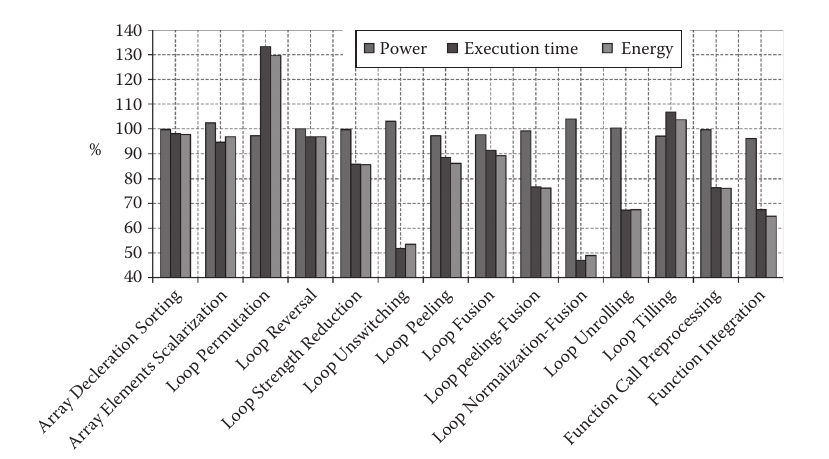
\includegraphics[scale=0.4]{graph.png}
\end{frame}

\begin{frame}
\frametitle{Dubbi}
\begin{itemize}
\item Target architecture.
\item Periferiche.
\item Regole già presenti.
\end{itemize}
\end{frame}

\end{document}